%%%%%%%%%%%%%%%%%%%%%%%%%%%%%%%%%%%%%%%%%%%%%%%%%%%%%%%%%%%%%%%%%%%%%%%%%%%%%
\chapter{Hauptteil}
\label{chap:intro}
%%%%%%%%%%%%%%%%%%%%%%%%%%%%%%%%%%%%%%%%%%%%%%%%%%%%%%%%%%%%%%%%%%%%%%%%%%%%%
\chapterstart

\section{Theoretischer Hintergrund:}

In diesem Kapitel soll eine Basis für die Grundlegenden Technologien, Standards und Begriffe geschaffen werden, welche im Zuge der wissenschaftlichen Arbeit verglichen bzw. verwendet wurden.

Die Arbeit Untersucht die Kommunikation zwischen Frontend zu Backend Komponenten, im industriellen als auch wissenschafltichem Kontext sind diese Begriffe wie folgt definiert:

\chapquote{"Das Frontend ist das, was Ihre Benutzer sehen, und enthält visuelle Elemente wie Schaltflächen, Kontrollkästchen, Grafiken und Textnachrichten. Es ermöglicht den Benutzern, mit Ihrer Anwendung zu interagieren. Das Backend sind die Daten und die Infrastruktur, die dafür sorgen, dass Ihre Anwendung funktioniert. Es speichert und verarbeitet Anwendungsdaten für Ihre Benutzer.“}
{\cite{awsfrontendbackend}}

Wie aus dieser Definition ersichtlich beinhaltet das Front-End den benutzerspezifischen Teil und das backend den Datenverarbeitungsteil. Im Zuge der Bachelorarbeit werden anschlieden für die Front End Komponente ebenso das Wort „Client“ und für die Backend Komponente das wort „Server“ verwendet.

\subsection{Serialisierungsformate}
Bei der Übertragung zwischen der Front-End und Back-End Komponente werden Daten ausgetauscht. Da es eine Vielzahl an Technologien gibt, mit denen die jeweiligen Komponenten realisiert werden können, wurden Standards definiert, damit diese sinnvoll und effizient verarbeitet werden können.

\subsubsection{JSON}
JSON steht für JavaScript Object Notation und ist ein weit verbreitetes, textbasiertes Datenformat, das vorallem wegen einfacher Lesbarkeit und breiter Unterstützung in vielen Programmiersprachen Verwendung findet. Das Format basiert auf einer Schlüssel-Wert Paar Struktur mit einfacher Syntax ( Klammern, Spalten, Doppelpunkte, Kommas ) und kann folgende Datentypen annehmen:

\begin{itemize}
	\item String (Zeichenkette)
	\item Number (Zahl)
	\item Boolean (true/false)
	\item Array (Liste)
	\item Object (Objekt mit weiteren Schl\"ussel-Wert-Paaren)
	\item null (leerer Wert)
\end{itemize}


JSON ist der Standard für REST und GraphQL Schnittstellen.


\subsubsection{Protocol Buffers}
Protocol Buffer sind ein von Google entwickeltes Serialisierungsformat. Es handelt sich hierbei um ein binäres Serialisierungsformat, das entwickelt wurde um möglichst effizient, mit hoher Performance und mit so wenig Overhead wie möglich (ohne Whitespaces oder Satzzeichen wie bei JSON) Daten zu übertragen und zu verarbeiten. Protocul Buffer sind Plattform unabhängig und mit den meisten gängigen Programmiersprachen kompatibel.
Ein zentraler Bestandteil Protocol Buffer sind dabei plattformunabhängigen .proto Files, die für die Erzeugung definiert werden müssen.

Mit den definierten .proto Files können anschließend mit einem Plattform Abhängigen Protobuf-Compiler-Tool ( z.B. protoc ) Datenobjekte der jeweiligen Programmiersprache generiert werden.


\newpage
\textbf{\underline{Aufbau der .proto Files}}
\newline
Hauptbestandteil der .proto Files sind messages und services.

\begin{verbatim}
	message Person {
		string name = 1;
		int32 id = 2;
		string email = 3;
	}
\end{verbatim}

Messages geben dabei die Struktur der zu übertragenden Nachricht und den jeweiligen Datentypen an und einer Nummer, die beschreibt an welcher Stelle sich das jeweilige Attribut befindet, an. Die Nummerierung der Felder ist wichtig für die Serialisierung.
In Protocol Buffers können unter anderem die gängigsten Datentypen wie int32, int64, float, double, bool sowie string und bytes verwendet werden.

\begin{verbatim}
	service PersonService {
		rpc GetPerson (PersonRequest) returns (Person);
	}
\end{verbatim}

Services geben an, welche Dienste vom Server bereit gestellt werden und welche Datentypen als Parameter bei Aufruf übermittelt und als Rückgabe zurückgegeben werden. Services müssen auf der Seite des zur Verfügung stellenden Dienstes ausimplementiert werden.

Das Protobuf Serialisierungsformat wurde vorallem für die inter-server Kommunikation ( innherhalb der Backend seitigen Kommunikation) entwickelt, im Zuge der Bachelorarbeit wird diese auf die Verwendung in der Frontend zu Backend Kommunikation untersucht.

\subsection{Transportprotokolle}
Die eigentlichen Daten, die in Form von Serialisierungsformaten zwischen Frontend und backend ausgetauscht werden, werden mithilfe von Transportprotokollen von dem Client and den Server, und umgekehrt, übermittelt. Das Hypertext Transfer Protocol (http) ist dabei für moderne Webanwendungen das zentrale und verbreitetste Transportprotokoll. Im Kontext der Bachelorarbeit, wird insbesondere auf zwei Versionen von http eingegangen:

\subsubsection{HTTP/1.1}

http/1 Ist der momentan am weitesten verbreitetste Protokoll für die Kommunikation zwischen Frontend und Backend anwendungen. Es wird von allen Webbrowsern ohne einschränkungen unterstützt und bildet die Grundlage für die API Technologien REST und GraphQL. Das Protokoll funktioniert mittels eines request-responds Prinzips und überträgt die Daten über eine textbasierte Verbindung mittels eines TCP Transportprotokolls. 

\begin{figure}[htbp]
	\centering
	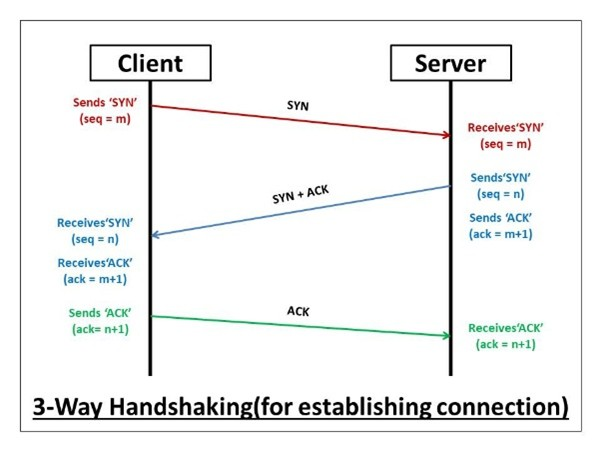
\includegraphics[width=0.7\textwidth]{images/http1_theory.jpg}
	\caption{3-Way Handshake (for establishing TCP connection)}
	\label{fig:threewayhandshake}
\end{figure}

Der Verbindungsaufbau erfolgt dabei mittels eines Transmission Control Protocol  (TCP) – Handshakes, welcher für eine zuverlässige Verbindung zwischen zwei Systemen verwenden wird. Dabei werden in drei Schritten Steuerpakete ausgetauscht:

1. Zuerst sendet der Client ein SYN (Synchronize( – Paket an den Server
2. Der Server antwortet mit einem SYN – ACK ( Acknowledge) Paket
3. Der Cient antwortet mit einem ACK

Ernst nach diesen Schritten, gilt die Verbindung als aufgebaut und die Daten werden übertragen.

Vorallem wegen der sequentielle Abarbeitung  und die Notwendigkeit von mehreren Verbindungen bei parallelen Requests führt häufig zu Performance Einschränkungen, welche vorallem bei dantenintensiven Anwendungen zu Problemen führen kann. 


\subsubsection{HTTP/2}
Aufgrund der ber http/1 genannten Performance Problemen wurde eine neue Version namens http/2 Enwickelt, weche viele Schwächen von http/1.1, insbesondere beszogen auf Latenz und Effizienz, ausgleicht.
Das Hauptmerkmal von http/2 ist Multiplexing, hierbei ist es möglich mehrere parallele Anfragen und Antworten über nur eine einzige TCP-Verbindung durchzuführen.
Weitere Verbesserungen beinhalten zum Beispiel die Komprimierung von Header-Informationen oder das Server Push-Verfahren, das eine proaktive Übertragung vom Server an den Client erlaubt.
Aufgrund der oben genannten Verbesserungen wird http/2 besonders in modernen Anwendungen in denen eine schnelle und effiziente Datenübertragung wichtig ist, wie biespielsweise bei gRPC, Echtzeitkommunikation oder Microservices verwendet.
Webbrowser unterstützen nur eine eingeschränkte Nutzung von http/2 deshalb können bei der Kommunikation zwischen Webbrowsern und Serveranwendungen nicht alle Vorteile ausgenutzt werden. Zwar unterstützen aktuelle Webbrowser mittlerweile http/2, jedoch ist bei der verwendung eine verschlüsselte Übertragung verpflichtend, und wichtige Features wie echted bidirektionales Streaming (gleichzeitiges Senden und Empfangen von Daten durch Client und Server) oder http/2 Trailers (das Übermitteln zusätzlicher Metadaten am Ende einer Übertragung, zum Beispiel zur Fehlerbehandlung, welche bei gRPC zum einsatz kommen, werden in Webbrowsern nicht bzw. nur teilweise unterstützt. Dadurch können bei der Kommunikation zwischen Frontend (Webbrowser) und Backend nicht alle Potenziale von HTTP/2 ausgeschöpft werden 

\subsection{API-Technologien}
API Technologien wie REST, GraphQL oder gRPC sind Schnittstellen, durch welche eine Kommunikation mit anderen Kommunikationspartnern möglich ist. Diese API-Technologien legen Standards fest ( Konventionen, Art der Serialisierungsobjekte, Art des Transportprotokolls) die neben der technischen Kompatibilität für die Kommunikation auch Entwicklern hilft, sich effizient in API-Systemen zurecht zu finden.
\subsubsection{REST}
\subsubsection{GraphQL}
\subsubsection{gRPC}
\subsection{Begriffe}
\subsubsection{Latenz}

\chapterend

